\documentclass[tikz,border=12pt]{standalone}
\usepackage{xcolor}
\usepackage{newpxtext,newpxmath}
\usepackage{pgfplots}
\pgfplotsset{compat=1.18}
\usetikzlibrary{calc, positioning}

% Color Palette matching template.tex
\definecolor{SitePrimary}{RGB}{165, 124, 117}
\definecolor{DarkCharcoal}{HTML}{2B2B2B}
\definecolor{LightTaupe}{RGB}{245, 242, 240}
\definecolor{SubtleGray}{HTML}{F4F4F4}
\definecolor{BarGray}{HTML}{B0BEC5}
\definecolor{BarDark}{HTML}{546E7A}

\begin{document}
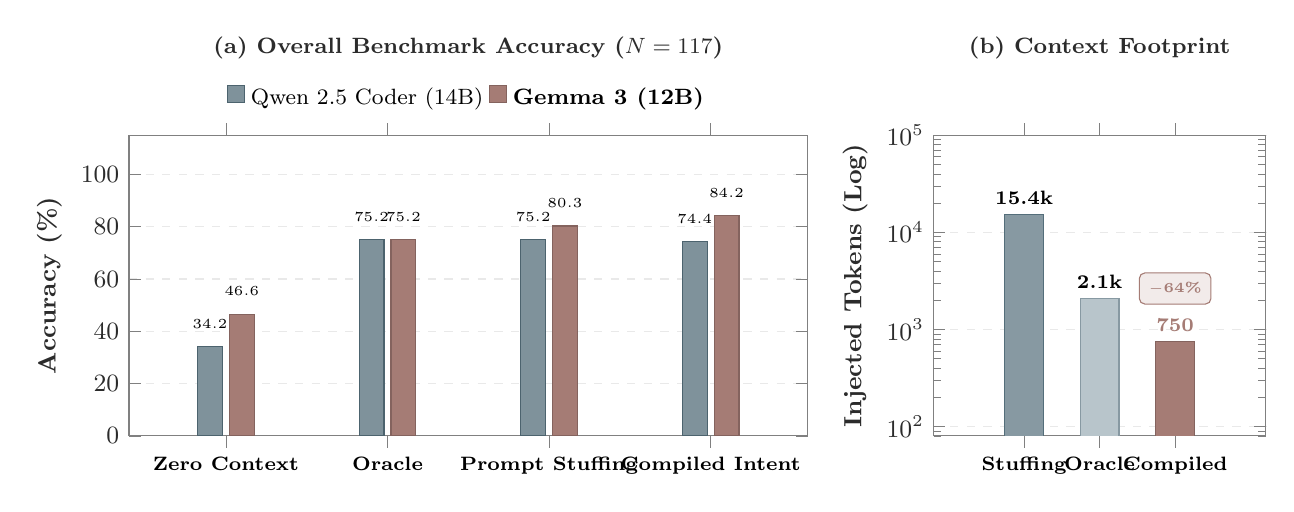
\begin{tikzpicture}[font=\small\color{DarkCharcoal}]

    % --- Left Plot: Overall Accuracy across Architectures ---
    \begin{axis}[
        name=accuracyPlot,
        ybar=2.5pt,
        bar width=9pt,
        width=10.2cm,
        height=5.4cm,
        title={\bfseries (a) Overall Benchmark Accuracy ($N=117$)},
        title style={font=\footnotesize\bfseries\color{DarkCharcoal}, yshift=18pt},
        ylabel={\bfseries Accuracy (\%)},
        ymin=0,
        ymax=115,
        ytick={0, 20, 40, 60, 80, 100},
        symbolic x coords={Zero, Oracle, Stuffing, Compiled},
        enlarge x limits=0.2,
        xtick=data,
        xticklabels={Zero Context, Oracle, Prompt Stuffing, Compiled Intent},
        x tick label style={font=\scriptsize\bfseries},
        nodes near coords,
        nodes near coords style={
            font=\tiny\bfseries,
            /pgf/number format/fixed,
            /pgf/number format/precision=1,
            /pgf/number format/zerofill
        },
        every node near coord/.append style={yshift=3pt},
        legend style={
            at={(0.5, 1.05)},
            anchor=south,
            legend columns=2,
            draw=none,
            fill=none,
            font=\footnotesize
        },
        legend image code/.code={
            \draw[#1] (0cm,-0.06cm) rectangle (0.22cm,0.16cm);
        },
        axis line style={DarkCharcoal!60},
        tick style={DarkCharcoal!60},
        ymajorgrids=true,
        grid style={dashed, SubtleGray!60!black!20}
    ]
        % Qwen 2.5 Coder 14B
        \addplot[fill=BarDark!75, draw=BarDark!90!black] coordinates {
            (Zero, 34.2)
            (Oracle, 75.2)
            (Stuffing, 75.2)
            (Compiled, 74.4)
        };
        \addlegendentry{Qwen 2.5 Coder (14B)}

        % Gemma 3 12B
        \addplot[fill=SitePrimary, draw=SitePrimary!80!black] coordinates {
            (Zero, 46.6)
            (Oracle, 75.2)
            (Stuffing, 80.3)
            (Compiled, 84.2)
        };
        \addlegendentry{\bfseries Gemma 3 (12B)}

    \end{axis}

    % --- Right Plot: Token Payload on Log Scale ---
    \begin{axis}[
        name=tokenPlot,
        at={($(accuracyPlot.east)+(1.6cm,0)$)},
        anchor=west,
        ybar,
        bar width=14pt,
        every axis plot/.append style={bar shift=0pt},
        width=5.8cm,
        height=5.4cm,
        title={\bfseries (b) Context Footprint},
        title style={font=\footnotesize\bfseries\color{DarkCharcoal}, yshift=18pt},
        ymode=log,
        log basis y=10,
        ylabel={\bfseries Injected Tokens (Log)},
        ymin=80,
        ymax=100000,
        symbolic x coords={Stuffing, Oracle, Compiled},
        enlarge x limits=0.6,
        xtick={Stuffing, Oracle, Compiled},
        xticklabels={Stuffing, Oracle, Compiled},
        x tick label style={font=\scriptsize\bfseries},
        axis line style={DarkCharcoal!60},
        tick style={DarkCharcoal!60},
        ymajorgrids=true,
        grid style={dashed, SubtleGray!60!black!20}
    ]
        % Stuffing Tokens
        \addplot[fill=BarDark!70, draw=BarDark] coordinates {(Stuffing, 15400)}
            node[above, font=\scriptsize\bfseries] {15.4k};
        
        % Oracle Tokens
        \addplot[fill=BarGray!90, draw=BarDark!70] coordinates {(Oracle, 2100)}
            node[above, font=\scriptsize\bfseries] {2.1k};

        % Compiled Intent Tokens
        \addplot[fill=SitePrimary, draw=SitePrimary!80!black] coordinates {(Compiled, 750)}
            node[above, font=\scriptsize\bfseries\color{SitePrimary}] {750};

        % Reduction annotation badges
        \node[fill=SitePrimary!15!white, draw=SitePrimary, rounded corners=2pt, font=\tiny\bfseries\color{SitePrimary}, anchor=south] at (axis cs:Compiled, 1800) {$-$64\%};

    \end{axis}

\end{tikzpicture}
\end{document}
